\subsection{GangaliaSink32}

\begin{figure}[h!]
  \caption{Metric2}
  \centering
    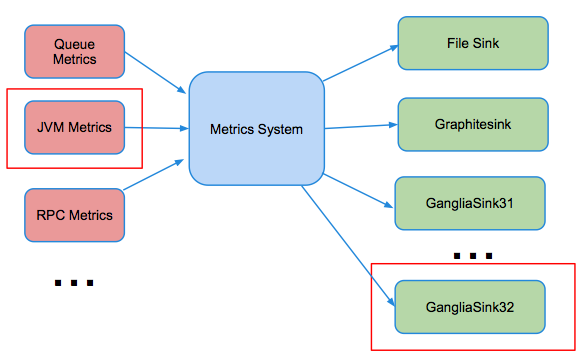
\includegraphics[width=0.5\textwidth]{image/ganglia32}
\end{figure}

\subsection{Ganglia Filter}

We found that Ganglia keeps to report finished task's metric as the last value it received. It makes the reported memory usage in a machine incredible large because the finished task memory usages are all counted into the sum of memory usage.

We added a filter inside the Ganglia API server to clean out the metrics of finished tasks. If one metric is continual reported as same value over tolerated period $T$, the filter will assume the task has finished, and remove the finished metric from reported API. 
